%- Quintile sorted predicted returns (simonian 2019)
%-OLS
% - summaries for coef attribution
%-RF
% - Summary for feat imp
% compare coefficients between feat imp and ols coef
% Sector rotation strat

\subsection{Hypothesis}

The aim of this subsection is to formalise ex ante hypotheses concerning the predictive accuracy and interpretability of all OLS and RF variations. 

We first consider the OLS base models. I speculate that within the estimation window, all factors in both the C4F and FF5 sets will attain statistical significance at the 5\% level when explaining monthly excess returns, yielding in\-sample $R^{2}$ values of at least 0.35.  This expectation is based on the well\-established risk\-pricing role of each factor: market excess return ($R_{M}-R_{f}$) as the primary driver per the Capital Asset Pricing Model, size ($SMB$) and value ($HML$) premia from \citeA{ff3_1993} foundational empirical findings, and the momentum effect ($UMD$) extended by \citeA{cahart_1997}. In the FF5 context, profitability ($RMW$) and investment ($CMA$) factors are likewise anticipated to be positively signed and signifitcant consistent with \citeA{novymarx_2013} Nevertheless, we expect the predictive $R^{2}$ out of sample to not be too low despite the inability of a static OLS framework to adapt to evolving market regimes (e.g.\ shifts in liquidity, sentiment, or sectoral leadership). An equity excess returns is usually not too wildly volatile (as we would see in section \ref{sec:data}), therefore it would not be too volatile to predict. %improve this in 2nd draft

%['vol', 'ret', 'shrout', 'prc', 'askhi', 'bidlo', 'put_volume','call_volume', 'put_call_ratio', 'vix_close', 'turn','zero_trade_ratio', 'baspread', 'mktrf', 'smb', 'hml', 'rmw', 'umd','cma', 'rf', 'enhanced_baker', 'news_sent', 'mktcap', 'turn_sd','sect_mktcap', 'mvel1', 'dolvol', 'daily_illq', 'excess_ret','excess_mkt_ret']

OLS enhanced models, due to possible multicollinearity among regressors inflating variance inflation factors and coefficients, I hypothesize that most of the Liquidity and Sentiment factors will remain statistically insignificant.  Consequently, I anticipate that only the original C4F factors (and market excess return in particular) will retain reliable significance, while overall in\-sample and out\-of\-sample $R^{2}$ will decline relative to the base OLS models. Therefore, OLS enhanced models is hypothesized to yield less accurate predictions.

The exceptionally turbulent market conditions of 2018 would exacerbate the limitations of linear OLS models, particularly in sectors such as Real Estate and Communication Services where idiosyncratic drivers dominate. In these conditions and certain segments, asset returns often exhibit behaviours that are macroeconomic dependent and nonlinear drawdowns that violate the constant-beta and homoskedasticity assumptions underlying OLS, which I hypothesize would yield biased forecasts and poor risk-adjusted performance. Consequently, while the expanded factor set may capture more risk dimensions, it is undermined by both linear model misspecification and the market conditions.

RF regression models offer a compelling non-parametric alternative to OLS by relaxing the linearity and additivity assumptions inherent in OLS. As an ensemble of decision trees, RF can capture nonlinear relationships and high order interactions among predictors without requiring an exact functional form. I therefore hypothesise that, when applied to monthly excess-return forecasting, RF will achieve both a higher in-sample $R^2$ and lower out-of-sample MSE than comparable OLS specifications. RF mitigates overfitting through bootstrap aggregation and random feature subsampling, so long as tuning parameters (tree depth, number of trees, minimum node size) are selected via cross-validation or out-of-bag error minimisation.

Nevertheless, the flexibility of RF does not guarantee uniform improvements across all forecasting Fama-French variations and enhancements. While RF inherently down weights irrelevant or redundant predictors through its random bootstrapping mechanism, deep trees can still split on spurious patterns or overfit if hyperparameters are poorly specified. We therefore anticipate that, under strict point forecast metrics or in macroeconomic situations that have low signal-to-noise ratio, an OLS model may outperform a naively tuned RF baseline. Still, for volatile and high growth sectors such as Real Estate where return drivers exhibit threshold effects, regime dependent nonlinearities, and intricate macro micro interactions RF's adaptive partitioning will yield substantial gains in predictive accuracy relative to linear models. Furthermore, due to the Random Forest specification, including a broad array of liquidity risk and sentiment proxies will not harm and even enhance—RF's forecasting performance, in stark contrast to the coefficient instability induced by multicollinearity in OLS. Because each tree in the forest sees only a random subset of predictors at each split, correlated or redundant features are unlikely to dominate model variance, and the ensemble average remains stable. In terms of attribution, RF FI metrics (e.g., permutation importance or SHAP values) are expected to convey the same principal drivers of excess returns as OLS $t-statistics$, albeit without formal inferential guarantees such as confidence intervals or $p-values$. Thus, while RF output richer insights into interaction effects and nonlinear contributions, its interpretability must be framed in predictive terms

\subsection{Model Interpretability: A Critique of pseudo-beta}

% - \citeA{simonian_2019} claimed that this could be a good substitute that could help communicate between machine learning models and finance people with a pseudo beta. However, with this data set and with the methods implemented, pseudo beta is unnlikely to be able to translate the findings of Random Forest into actual betas that are able to explain the returns of the assets.

% - It is found that, on all significant instance of any OLS coefficent of variables, RF is always off by 50\% or more. In some cases, we can see a 200 \% difference between the RF and OLS beta.

% - THerefore the notion of attempting to translate between RF betas and OLS is meaningless: This inconsistency goes against the notion of beta for financial experts: have a clear understanding of the drivers of returns and the ability to translate the findings of Random Forest into actual betas that are able to explain the drivers of the assets. Inconsistencies between these models muddy the water, and it does not have a statistical backing of t-tests.

% - However, though for attribution OLS is a better choice, for forecasting tools available are much more diverse and helpful. the magnitude of any variable effect could still be observed through SHAP, PDP and permutation importance so that finance professionals could still have a clear understanding of the drivers of returns.

\citeA{simonian_2019} originally proposed the concept of a “pseudo-beta” as a bridge between the predictive strengths of RF and the familiar beta coefficients derived from OLS, arguing that weighting RF variable importances by feature elasticity could yield interpretable analogues of linear factor loadings. However, when applied to our dataset and estimation procedures, the pseudo-beta approach fails to produce pseudo betas that are both numerically accurate and statistically reliable. Specifically, for every explanatory variable exhibiting a statistically significant OLS coefficient, the corresponding RF-derived pseudo-beta diverges from its OLS counterpart by at least 50\%, and in extreme cases by over 200\%. Such large discrepancies indicate that the pseudo-beta does not faithfully translate the nonlinear sensitivities learned by RF into the linear elasticity framework expected by financial practitioners. Therefore, OLS based factor models are still more appropriate to derive finance betas and answer questions such as "How many percent increase in excess returns can we expect if an increase in by 1\%?".

This inconsistency fundamentally undermines the utility of pseudo-beta as an interpretability tool: it contradicts the core financial utitlity that “beta” convey a stable measure of an asset's sensitivity to risk factors, complete with statistical rigor proof via $t$-tests. Instead of communicating with financial practicioners the drivers of returns, these unstable mappings only serve to “muddy the water” as the variability in pseudo-beta estimates lacks both statistical backing and economic coherence. Nonetheless, for forecasting applications, such as in this empirical study, practitioners are not without recourse. Model agnostic interpretability methods such as SHAP values, partial dependence plots (PDP) and permutation importance can still reveal the relative magnitude and direction of each feature's impact on predicted returns.

For example, if finance practictioners want to look into what drives excess returns the Real Estate sector RF-EN-C4F model, they could look at SHAP values, Partial Dependence Plot (PDP) and Permutation Importance. Below is an example of SHAP values for the RF-EN-C4F model, one of the highest performing sector rotaion model in this study. However, because attribution is not the primary objective of this study, rigorous validation of these effects and the identification of their true drivers remain outside its scope and warrant further investigation.

SHAP (SHapley Additive exPlanations) values measure each feature's contribution to the model's prediction for individual observations. In the SHAP plot (\cref{fig:rf_60_rf_enhanced_shap_plot}), the features are ranked by their average absolute impact on the prediction. For instance, high values of \texttt{mvell} are associated with positive SHAP values, which indicates that larger market value to earnings ratios tend to increase predicted excess return, whereas low values of \texttt{mvell} push predictions downward. Similarly, \texttt{vix\_close} exhibits a cluster of high excess returns with positive SHAP contributions, suggesting that higher market volatility also tends to raise the model's estimate of excess returns.

If they want a more granular and quantifiable effect of each variable on excess return, holding other features constant, they could look at PDP (\cref{fig:rf_60_rf_enhanced_rf_pdp}). It shows the effect each variable has on predicted excess returns, keeping other variables constant. For example, we could observe a monotonic increase in partial dependence as \texttt{vix\_close} rises from 15 to 35, suggesting that higher volatility increases predicted excess returns.

\begin{figure}[H]
    \centering
    \includegraphics[width=\textwidth]{plots/results/60_rf_enhanced_rf_pdp.png}
    \caption{Partial Dependence Plot of RF-EN-C4F model}\label{fig:60_rf_enhanced_rf_pdp}
\end{figure}

\begin{figure}[H]
    \centering
    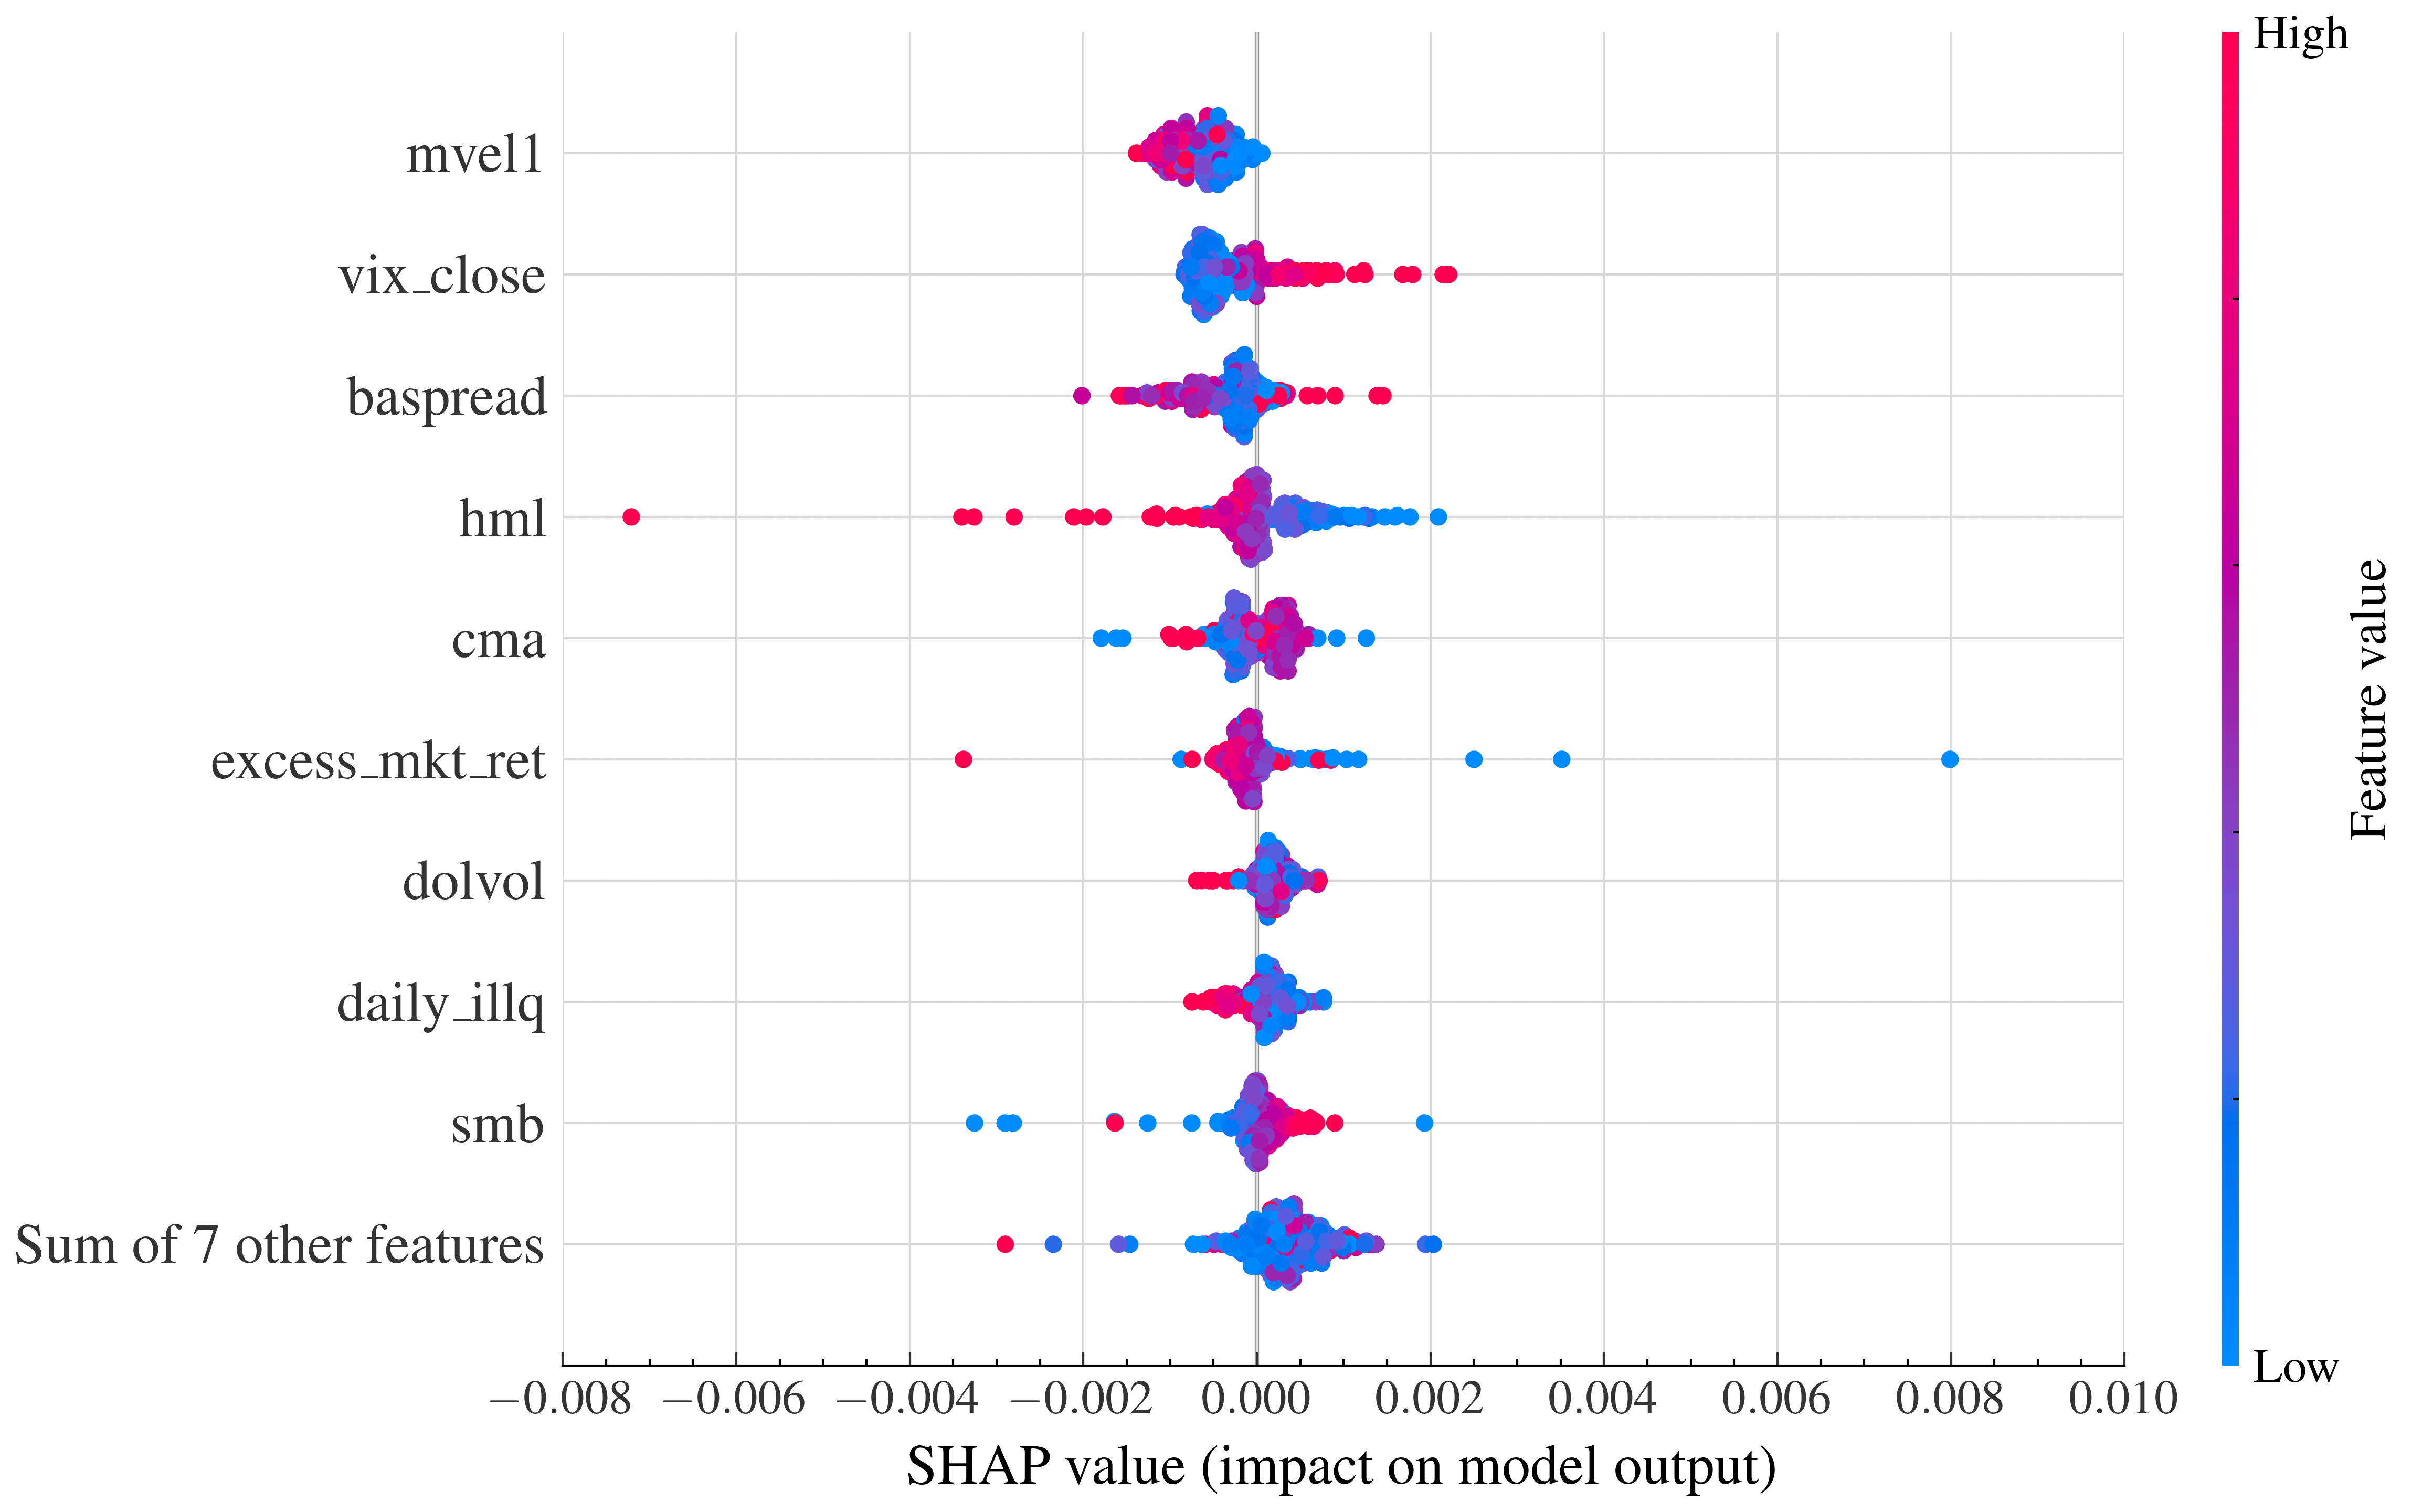
\includegraphics[width=\textwidth]{plots/results/60_rf_enhanced_shap_plot.png}
    \caption{SHAP values of RF-EN-C4F model}\label{fig:60_rf_enhanced_shap_plot}
\end{figure}




\subsection{Model Performance Comparison}
Forecasting performance is of paramount importance in this thesis, as it forms the foundation of our signal creation process. Models must be robust across all market conditions, whether facing high liquidity risk, volatility, or shifts in sentiment, to effectively hedge against potential losses. \cref{tab:baseline_ols_c4f,tab:baseline_ols_ff5,tab:enhanced_ols_c4f,tab:enhanced_ols_ff5,tab:enhanced_rf_c4f,tab:enhanced_rf_ff5,tab:rf_baseline_c4f,tab:rf_baseline_ff5} present the forecasting performance metrics for each model specification and factor variation.

- OLS Baseline: terrible fit (<1\% rsquared ). Though we see that the numerical values of mse, mae are quite tiny, we must remember that excess return is usually small below 0.001. Notably, for both c4f and ff5, sector 40 (fianncials) and especially 60 (real estate) did very poorly. Generally see no fitting for both Fama French variations with traditional OLS, but the RMSE hold indicates that they are not very robust in prediciting the 2018 hold out set. MAE does not tell us much due to it being very prone to outliers and this is a volatile hold out set.

- OLS enahnced: fit improve only marginally for both FF variations, however still terrible. Sector 40,60 performance have improved but still moedls are very prone to errors.

- RF base: Immediate significant imporvement in fit and in hould-out predictions. Surpring that sector 60, rf has the second lowest rmse hold out of all sector. Considering its volaitlity, this is massive win. One more surprise is that it seems like the more volatile the sector, the better the fit for C4F while it is the opposite for FF5, though this is marginal

- RF enhanced:Significanf fit increase, comparing to base. Again, we see that c4f is performing better than ff5 on sector 40 and 60, ff5 is more stable across all sectors. However, interesting thing to note that the forecast prediction performance itself does not differ too much from base.

\subsection{Sector Rotation Strategy}
We evaluate the sector rotation strategy over a hold-out sample comprising the calendar year 2018. The strategy's performance is benchmarked against the S\&P500 returns index, which is weighted by market capitalization, computed as the product of share price and total shares outstanding. Many empirical studies benchmark their investment or sector rotation strategies against the S\&P500 due to its status as the primary large-cap U.S. equity market proxy, such as \citeA{sawar_2017} where the authors uses S\&P500 as a benchmark for a sector rotation strategy using FF5 alphas. As detailed in \cref{sec:data}, 2018 was characterized by heightened market volatility and adverse macroeconomic shocks; consequently, the cumulative return of the S\&P500 over this period was $-6.24\%$ \footnote{This paper omits the data point on 30-12-2018 since on 30/12/2018, there are no next day signal to be used for forecasting (next trading day is on 2019). Therefore the reported returns is different. If this data point is included, the cumulative return of the S\&P500 over this period was $-6.24\%$ indeed.}.

To gauge risk-adjusted performance of the strategy, we report each portfolio's cumulative return, its active return relative to the S\&P500 (or 'Alpha'), and two spread sensitive statistics: the Information Ratio (IR) and the probabilistic Sharpe Ratio (PSR) at benchmark Sharpe thresholds $S^{*}=0$ and $S^{*}=0.1$. The IR evaluates excess return per unit of tracking-error volatility,

\begin{equation}
\mathrm{IR}=\frac{\mathbb{E}\left[R_{p}-R_{b}\right]}{\sigma\left(R_{p}-R_{b}\right)},
\end{equation}

where $R_{p}$ and $R_{b}$ are portfolio and benchmark returns, respectively, and a higher value signals more efficient investment relative to the risk taken by the investor. For example, an IR of below 0.1 means the strategy generates less than 0.1 units of excess return per unit of tracking error volatility, signaling that its returns are too small relative to their risk to justify strategy implementation. The PSR estimates the posterior probability that the true Sharpe ratio of a strategy exceeds a user-defined benchmark $S^{*}$,

\begin{equation}
\mathrm{PSR}= \Phi\left[\frac{\left(\hat{S}-S^{*}\right)\sqrt{T-1}}{\sqrt{1-\hat{S}^{2}/2}}\right],
\end{equation}
with $\hat{S}$ the sample Sharpe, $T$ the number of observations, and $\Phi(\cdot)$ the standard-normal cdf. Following \citeA{simonian_2019}, we report the PSR at $S^{*}=0$ and $S^{*}=0.1$.

The cumulative-return chart in \cref{fig:cum_ret_plot} together with the summary statistics in \cref{tab:return_stats_1} shows the effectiveness of the active sector-rotation strategies relative to a passive S\&P 500 benchmark buy and hold strategy. While the index declined by 7.03\% over 2018\footnote{Due to ommitted data on 30/12/2018, 2018 period ends on 29/12/2018.}, 7 out of 8 models specifications outperformed the S\&P500 index, and 4 out of 8 specifications made positive returns despite the market conditions. The plot further shows that these active portfolios not only outperformed during the steady upswing through September but also sucessfully adjusted to the sudden sell off and increased volatility from mid-October onward, thereby dampening the loss.

% A closer inspection reveals three surprises. 

% - First, the top three performers are all RF specifications, yet the fourth-best is an OLS specification. RF-C4f-EN is the best specification, achieving a cumulative return of 5.19\%, translating into an alpha of 12.31\%, an IR of 0.29 and a PSR of 0.97 at the 0.0 Sharpe benchmark. 

% Second, among RF models the base FF5 variant outperforms its liquidity-and-sentiment-enhanced variant. Opposite to that, rf_base_c4f lost money and performed worse than ols_en_ff5, while its enhanced c4f version is the best performing model.

% At the opposite end, the only portfolio that trailed the benchmark was the purely linear \texttt{ols_base_ff5} (-10.66\%), confirming that both non-linearity and the additional liquidity-sentiment layer are crucial when momentum is missing.

% - Incredible results. Looking at the fig we could see that almost all of  the active strategies are outperforming the buy and hold index strategy. First four models, in a year where Sp500 index loses 7.03%, our strategy were able to hedge against that and even made positive returns. Only one model out of 8 lost against the index
% - In the fig we see that even  the plunge from mid october and volatile times at the end of the year , our models adjusted to that extremely well and generate signals that could hedge against the liquidity risk and sentiment shift
% - Looking closer: top 3 models are rf specification, but extremely surprising that 4rth is ols. Looking deeper in the top 4, c4f enhanced performed best with the cummulative ret =5.19\%, achieving an active return of 12.31\% . surprising that c4f is on top not ff5 {WHY DO YOU THINK c4f is on top not ff5}. even more surprising is that rf_base ff5 seems to beat rf_enhanced_ff5. {WHY IS THIS THE CASE}, with 11.44 active return comapred to 10.65\% active return. Most surpirasing of all, however, is that the 4rth place is not rf but an ols model, specifically ols_en_ff5 {WHY IS THIS POSSIBLE?}

% - Bottom 4 models: rf_base_c4f lost money {WHY enhanced do so good but base lost?}. Contrary to the hypothesis, ols base models performed worse than the ols enhanced, specifically c4f >ff5. Ols_base ff5 is the only one that lost money {WHY?}


\begin{figure}[H]
    \centering
    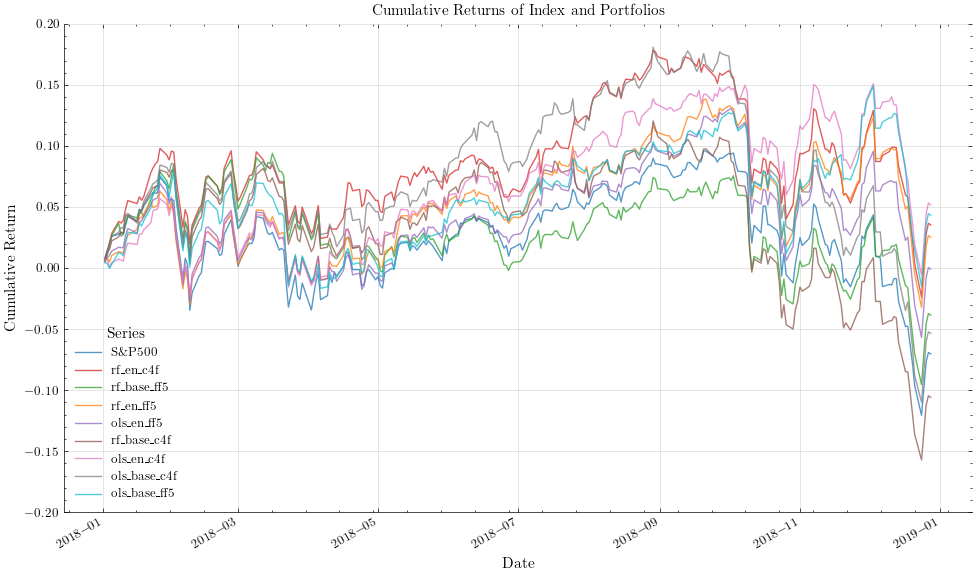
\includegraphics[width=\textwidth]{plots/results/cum_ret_plot.png}
    \caption{Cumulative returns of S\&P500 and sector rotation strategies (2018)}\label{fig:cum_ret_plot}
\end{figure}



\begin{table}[ht]
\centering
\caption{Descriptive Statistics of Index and Portfolio Returns}
\label{tab:return_stats_1}
\begin{tabular}{lrrrrrrr}
\toprule
{} & \multicolumn{1}{c}{Cumulative} & \multicolumn{1}{c}{Annualised} & \multicolumn{1}{c}{Annualised} & \multicolumn{1}{c}{Alpha} & \multicolumn{1}{c}{Information} & \multicolumn{1}{c}{PSR} & \multicolumn{1}{c}{PSR} \\
{} & \multicolumn{1}{c}{Return} & \multicolumn{1}{c}{Return} & \multicolumn{1}{c}{Volatility} & {} & \multicolumn{1}{c}{Ratio} & \multicolumn{1}{c}{(S*=0)} & \multicolumn{1}{c}{(S*=0.1)} \\
\midrule
S\&P500 & -7.03\% & -7.08\% & 17.06\% & 0.00\% & -- & -- & -- \\
rf\_en\_c4f & 5.19\% & 5.23\% & 15.72\% & 12.31\% & 0.29 & 0.97 & 0.61 \\
rf\_base\_ff5 & 4.33\% & 4.36\% & 16.45\% & 11.44\% & 0.28 & 0.95 & 0.57 \\
rf\_en\_ff5 & 3.54\% & 3.57\% & 16.55\% & 10.65\% & 0.29 & 0.95 & 0.55 \\
ols\_en\_ff5 & 2.53\% & 2.55\% & 16.27\% & 9.63\% & 0.28 & 0.95 & 0.53 \\
rf\_base\_c4f & -0.08\% & -0.08\% & 16.10\% & 7.00\% & 0.26 & 0.93 & 0.48 \\
ols\_en\_c4f & -3.85\% & -3.89\% & 16.48\% & 3.20\% & 0.22 & 0.89 & 0.38 \\
ols\_base\_c4f & -5.34\% & -5.38\% & 17.23\% & 1.70\% & 0.21 & 0.86 & 0.33 \\
ols\_base\_ff5 & -10.58\% & -10.66\% & 17.14\% & -3.58\% & 0.15 & 0.78 & 0.22 \\
\bottomrule
\end{tabular}
\end{table}



